\section{The unified diagram}\label{sec:diagram}
\subsection{Objects, maps and statuses}
The diagram of \cref{fig:global} has two columns of objects. On the generative side: histories, swap classes, contents, endpoints, occurrence sets of integers, endpoint complexes and their Betti numbers, and the route complexes and counts of the history space of a fixed source and endpoint. On the collective side: rational states, their occurrence sets, their move complexes and primitive systems, and the same data at the image under $C$. Integers belong to both sides.

Every arrow carries one of five statuses (see \cref{sec:intro} for the line conventions): \emph{established arrow} (a source-defined function, cited or defined here); \emph{proved factorization} (a map that factors through another under stated hypotheses); \emph{proved obstruction} (a reconstruction ruled out by an exact result); \emph{open construction}; \emph{interpretive comparison} (no formal correspondence claimed).
\subsection{Factorizations}
\cref{fig:fact} shows the factorization chain of \cref{sec:numerical,sec:occurrence} with the sets on which it is defined: the maps $\mathrm{Hist}(m_0)\to\mathrm{Cls}\to\mathrm{Cont}\to\Z\to\{D\}$ are for a fixed source $m_0$ (or all integers in the last step), and $D\mapsto K(D)\mapsto\beta$ are functions of $D$ (\Src{III}{thm:R3T1a}). The two obstructions leaving this chain are the primitive system (\cref{prop:P2}(c)) and the history counts (\cref{prop:P5}).
\begin{figure}[t]\centering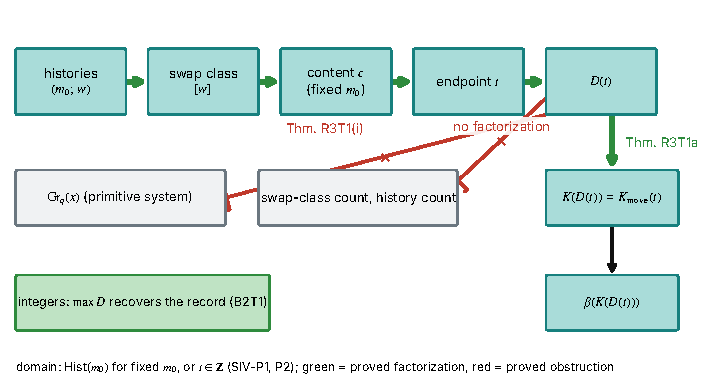
\includegraphics[width=\linewidth]{fig20_factorization_D.pdf}
\caption{\textbf{A source-supported factorization diagram.} What passes through the occurrence set $D$ and what does not. Green: proved factorizations; red: proved obstructions (\Src{III}{thm:R3T1}(i) and \cref{prop:P5}). \emph{Exact content: statuses and domains; boxes are schematic.}}\label{fig:fact}\end{figure}
\subsection{Commuting relations}
\begin{proposition}[no claimed commuting squares]\label{prop:nocomm}
Let $\iota:\Z\to\Q_{>0}$ be the inclusion. The following squares are \emph{not} claimed to commute and the corresponding statements are false or unestablished: (i) $C\circ\iota=\iota\circ T_N$ for any $N$ (false by \cref{prop:P9}(a); this excludes the identity-type correspondence only, not a non-identity $\Phi$); (ii) $K(D(\cdot))\circ\mathrm{end}$ determines the history complex (false by \cref{prop:P5}); (iii) $D\mapsto\Gr$ (does not exist, \cref{prop:P2}(c)). The only commuting relations proved in this manuscript are the factorization identities $\Endp=\pi_3\pi_2\pi_1$ and $\mathrm{(realised\ record)}=g\circ D$.
\end{proposition}
\begin{proof}
(i) is \cref{thm:cited-corr}(i). (ii) is \cref{prop:P5}. (iii) is \cref{prop:P2}(c). The two commuting identities are \cref{prop:P1}(a) and \Src{III}{thm:R3T1a}.
\end{proof}
\begin{figure}[p]\centering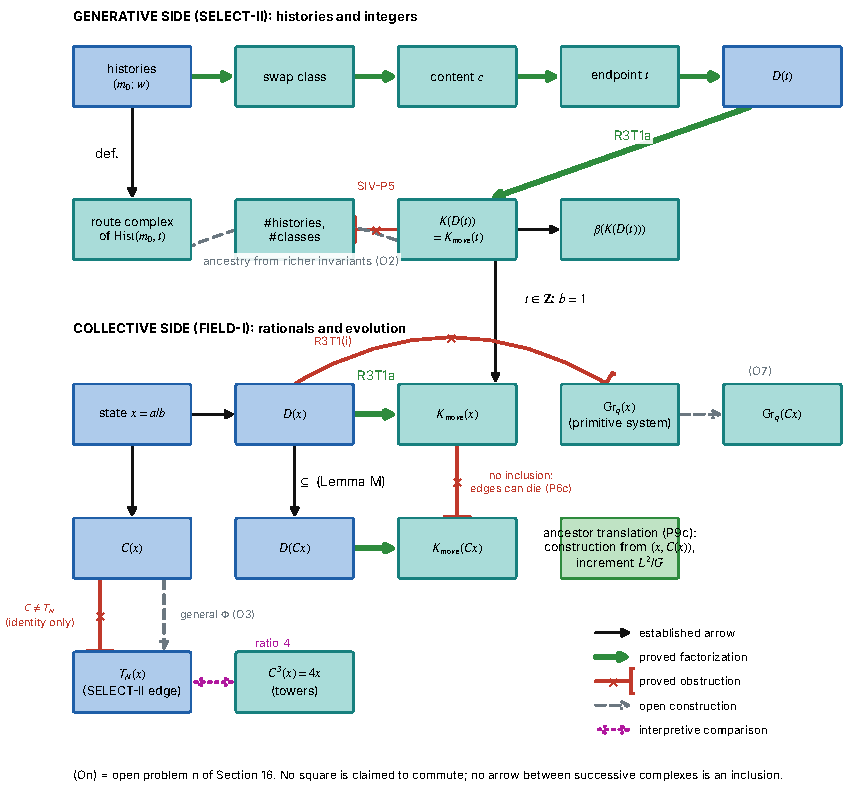
\includegraphics[width=\linewidth]{fig21_global_diagram.pdf}
\caption{\textbf{The global diagram of maps, factorizations and obstructions.} Objects are the structures of \cref{sec:objects}; each arrow is labelled with its status by line style and cited result. Green arrows: factorizations proved from the cited theorems; black arrows: established functions; red arrows with a cross: proved obstructions (R3T1(i) is \Src{III}{thm:R3T1}(i); SIV-P5 is \cref{prop:P5}; $C\ne T_N$ is \cref{prop:P9}(a)); grey dashed arrows: open constructions (O2, O3, O7); purple dotted arrow: interpretive comparison of the ratio $4$ (\cref{thm:cited-corr}(ii)). The arrow between $K_{\rm move}(x)$ and $K_{\rm move}(Cx)$ is drawn as an obstruction to an \emph{inclusion}: vertices persist but edges can be lost (\cref{prop:P6}(c)), so no complex inclusion is implied. The box \emph{ancestor translation} is a construction from the arithmetic pair $(x,C(x))$ and the set $D(x)$ (\cref{prop:P9}(c)), not a function of $K_{\rm move}(Cx)$, and is therefore drawn without an arrow from that complex. The legend is in the figure. \emph{Schematic of status: the diagram is a map of established relations, not a commuting diagram; the status of each arrow is defined in Appendix~\ref{app:diagram}.}}\label{fig:global}\end{figure}
